%!TEX root = Main_Assignment2.tex
\documentclass[Main_Assignment2]{subfiles}

\begin{document}
\section{Modeling the CPTAC using problem frames}


\begin{figure}[H]
\centering
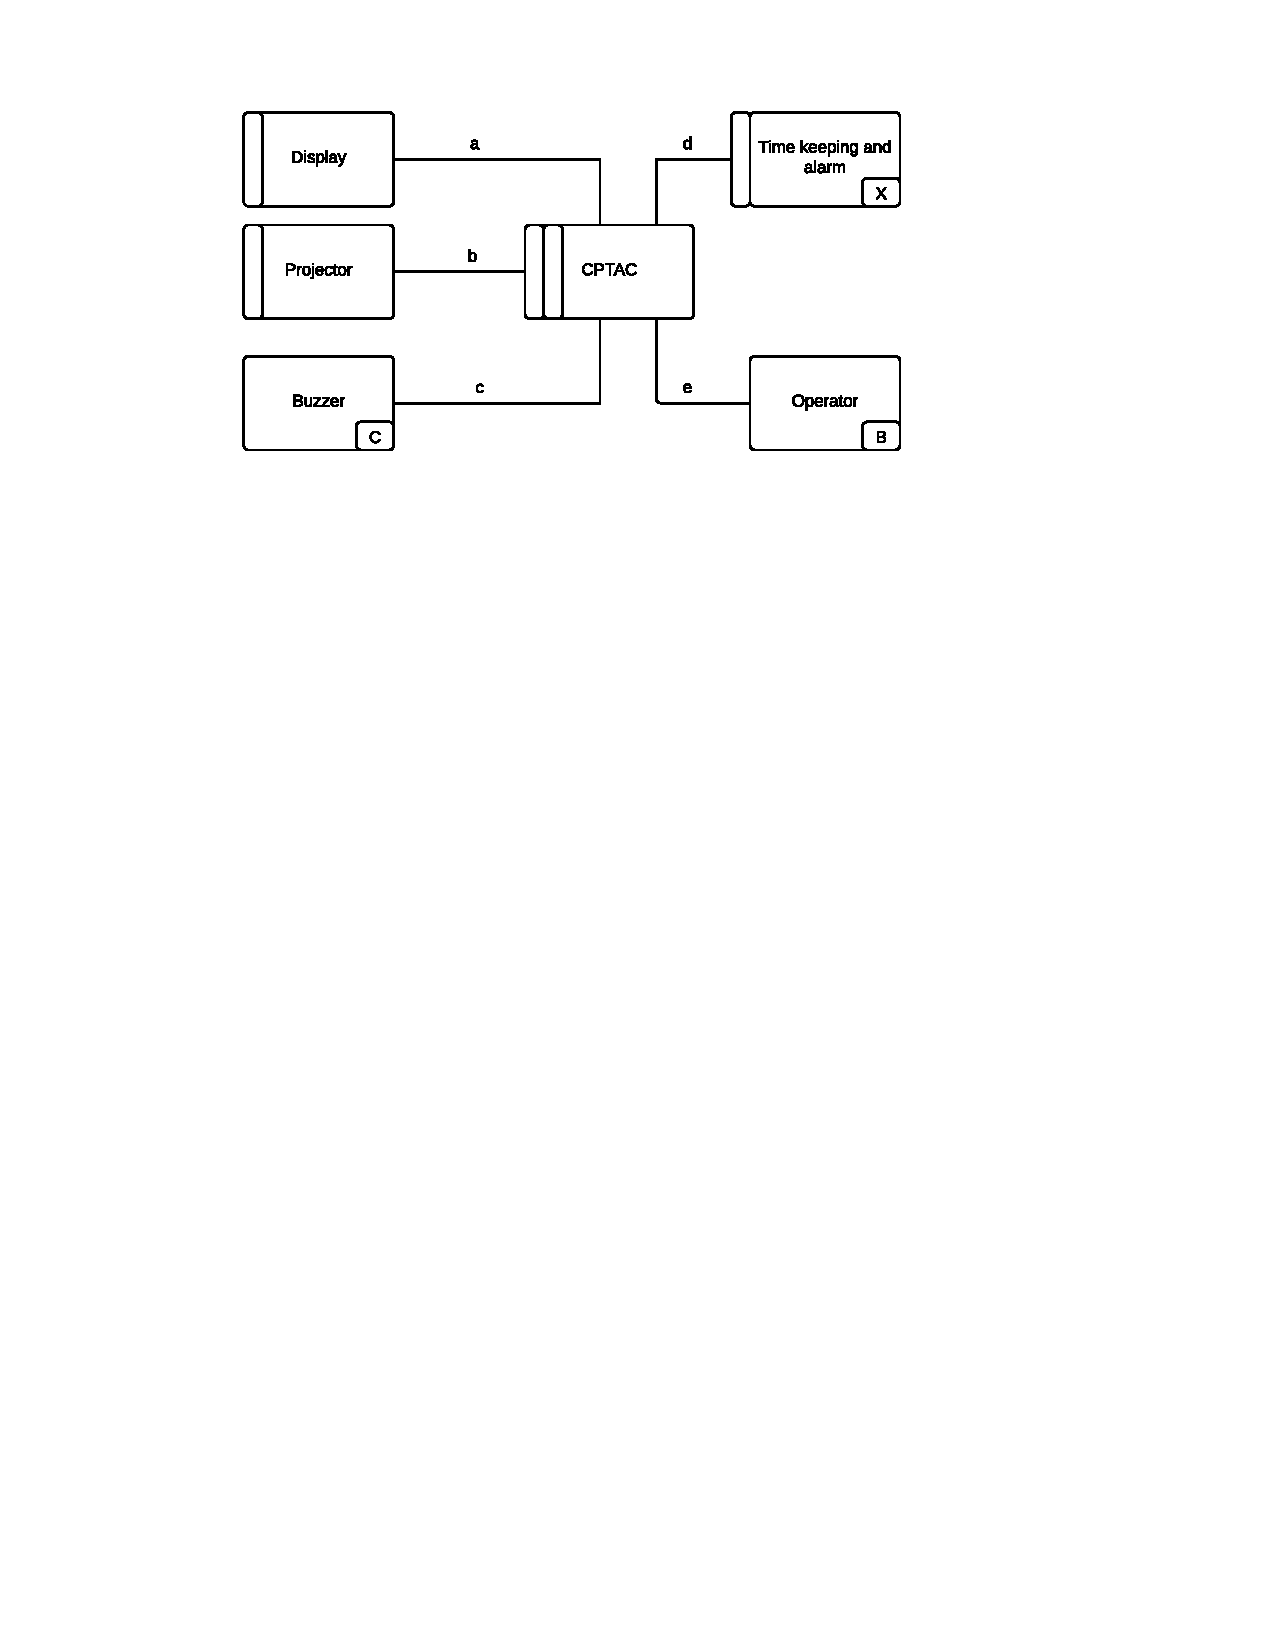
\includegraphics[width=0.8\linewidth]{ContextDiagram.pdf}
\caption{Context diagram}
\label{fig:contextDiagram}
\end{figure}

Description of interfaces in the context diagram and assignment of requirements:
\begin{enumerate}
	\item[a:] Show current time and alarm time: RE9, RE10, RE13, RE14, RE20
	\item[b:] Time projection: RE1, RE5, RE8, RE12, RE23
	\item[c:] SoundAlarm: RE4, RE21
	\item[d:] Time keeping: RE18, RE19, RE20, RE21
	\item[e:] Buttons: RE7, RE11-20, 
\end{enumerate}
	


\begin{figure}[H]
\centering
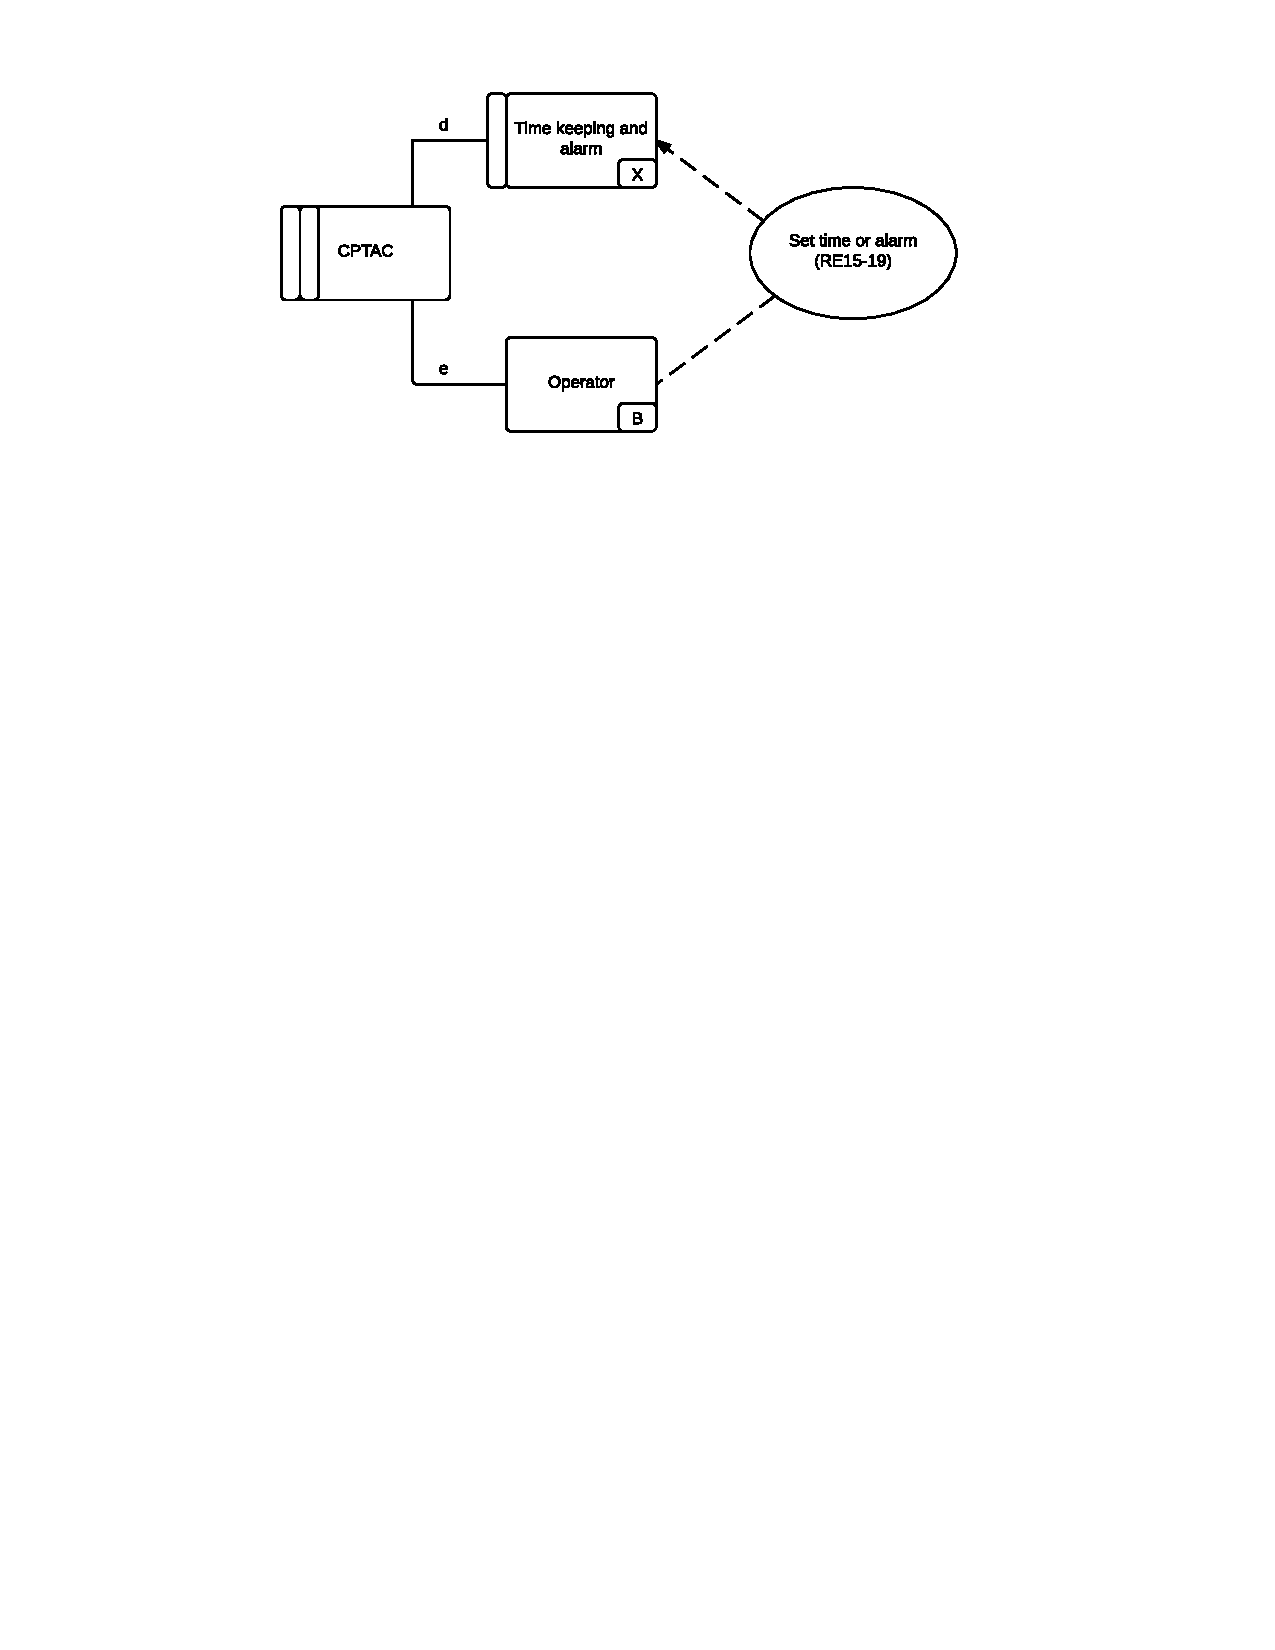
\includegraphics[width=0.7\linewidth]{ProblemFrame1.pdf}
\caption{Problem frame for setting time and alarm.}
\label{fig:problemFrame}
\end{figure}

\end{document}